\section{Streams}


\subsection{Grundlegendes}

\begin{frame}{Datenfluss}
	\begin{itemize}
		\item Container dienen zur Speicherung von Daten
		\item Streams dienen zum Versenden oder Empfangen von Daten\\
		      $\implies$ Datenfluss
		\item Meist entweder nur source (read-only) oder nur sink (write-only)
		\item Puffern von Datensequenzen vor/nach der Übertragung
		\item InputIterator (read-only, forward-only) für sources
		\item OutputIterator (write-only, forward-only) für sinks
	\end{itemize}
\end{frame}

\begin{frame}{Grundlegendes}
	Ein STL-Stream
	\begin{itemize}
		\item ist in erster Linie ein character-Streams
		\item nutzt im Hintergrund einen Puffer (\texttt{basic\_streambuf}-Derivat)\\
			$\rightarrow$ Der Puffer stellt die eigentliche Übertragungs-Funktionalität bereit!
		\item dient quasi nur der vereinfachten Nutzung des Puffers
		\item ist Zustands-behaftet z.B. für Eingabe mit fester Breite (\texttt{setw})
	\end{itemize}
\end{frame}


\begin{frame}{Locales}
	Unterschiedliche Konventionen in verschiedenen Ländern:
	
	\vspace{1em}
	
	\begin{tabular}{c|c|c}
		\textbf{USA}	&	\textbf{France}	&	\textbf{Deutschland}	\\
		\hline
		$3,042.12$		&	$3\;042,12$		&	$3\;042,12$				\\
		2:00 pm			&	14~h~05			&	14:00					\\
		June 22, 1996	&	22 juin 1996	&	22. Juni 1996			\\
	\end{tabular}
	
	\pause
	\vspace{0.5em}
	
	\begin{block}{Locale}
		Beschreibt in Facetten Regions-spezifische Aspekte des UI, z.B.
		\begin{itemize}
			\item Zahlenformatierung (facets: \texttt{num\_get}, \texttt{num\_put})
			\item Minuskel/Majuskel-Konversion (facet: \texttt{ctype})
			\item Datum/Zeit (facets: \texttt{time\_get}, \texttt{time\_put}, \dots)
			\item lexikographische Sortierung (facets: \texttt{collate}, \texttt{collate\_byname})
			\item \dots
		\end{itemize}
	\end{block}
\end{frame}

\begin{frame}[fragile]{Locales in C++}
	\alert{ An sich eigenes Thema! }
	
	\pause
	\vspace{2em}
	
	\begin{lstlisting}[escapechar=\$]
		#include <locale>
		
		char const* const locale_name = "...";	// implementation-defined!
		std::locale loc(locale_name);
		
		char Ue = std::toupper('$ü$', loc);	// Ue == '$Ü$'
		char foo = std::toupper('$ß$', loc);	// foo == '$ß$' [sic!]
	\end{lstlisting}
	
	\vspace{1em}
	Meist aber indirekte Verwendung, z.B. über Streams.
\end{frame}


\begin{frame}{class hierarchy}
	\includegraphics[width=\textwidth]{images/streams-class-hierarchy}
\end{frame}

\begin{frame}[fragile]{template parameters of streams}
	\begin{block}{Introducing: basic\_ios, Standard 27.4.4}
		\begin{lstlisting}
			template
			<
			    typename T_Char,
			    typename T_CharTraits = std::char_traits < T_Char >
			>
			class basic_ios;
		\end{lstlisting}
		
		\vspace{1em}
		
		\begin{description}[leftmargin=5em]
			\item[\texttt{T\_Char}] der zugrunde liegende Block-/Character-Datentyp
			\item[\texttt{T\_CharTraits}] \enquote{String}-Operationen und Eigenschaften von \texttt{T\_Char}
		\end{description}
	\end{block}
\end{frame}

\begin{frame}{\texttt{ios\_base} und \texttt{basic\_ios}}
	Hauptsächlicher Inhalt:
	\begin{itemize}
		\item Formattierungs-Status (z.B. \texttt{std::ios\_base::width} $\leftarrow$ \texttt{setw})	\\
			(üblicherweise mittels stream manipulators)
		\item Fehler-Zustand
		\item locale-Management
		\item Puffer-Ownership; Puffer lässt sich zur Laufzeit austauschen: \texttt{basic\_ios::rdbuf}
		\item Einführung von Konstanten und Typen
		\item \footnotesize (private storage)
		\item \footnotesize (callback registration)
	\end{itemize}
\end{frame}

\begin{frame}{Fehlerzustände von Streams}
	\footnotesize
	\begin{block}{Konstanten des Fehler-Zustands}
		% hack is quicker hacked than nice things are nicely done
		\begin{tabular}{rl}
			\texttt{0 == ios\_base::goodbit}	&	kein Fehler	\\
			\texttt{ios\_base::badbit}			&	\enquote{unheilbarer} Fehler	\\
			\texttt{ios\_base::failbit}		&	I/O Fehler (Formattierung oder Extraktion)	\\
			\texttt{ios\_base::eofbit}			&	Input hat das Dateiende erreicht (end-of-file)	\\
		\end{tabular}
	\end{block}
	
	\pause
	
	EOF bzw. eofbit ist kein Fehlerzustand des Streams selbt, jedoch kann EOF zu einem Fehlerzustand führen (z.B. wenn extrahiert werden soll).
	
	\vspace{1em}
	
	{\tt
	\begin{tabular}{rcl}
		\textnormal{\textbf{member function}}	&	\textnormal{\textbf{returns true if}}&	\textnormal{\textbf{meaning}}\\
		\hline
		good()	&	rdstate() == goodbit	&	\textnormal{stream ready (for extraction/insertion)}	\\
		fail()	&	failbit \textnormal{or} badbit \textnormal{set}	&	\textnormal{something went wrong}	\\
		bad()	&	badbit \textnormal{set}	&	\textnormal{stream is irrecoverably \enquote{damaged}} \\
		eof()	&	eofbit \textnormal{set}	&	\textnormal{stream is at the EOF (not ready)}	\\
		operator bool()	&	!fail()	&	\textnormal{everything went fine (EOF still possible!)} \\
		operator! ()	&	fail()	&	\textnormal{something went wrong} \\
	\end{tabular}
	}
	
	\pause
	\vspace{1em}
	
	Merke: \texttt{fail} $\subset$ \texttt{bad}: \texttt{fail} allein kann man nicht direkt erfragen
\end{frame}


\subsection{output stream}

\begin{frame}{\texttt{basic\_ostream} template}
	Hauptsächlicher Inhalt:
	\begin{itemize}
		\item formatted output, stream manipulator \enquote{interface}: \texttt{operator<<}
		\item unformatted output: \texttt{put}, \texttt{write}
		\item \texttt{flush}
		\item \texttt{sentry}-Klasse
	\end{itemize}
	
	\pause
	\vspace{2em}
	
	\begin{block}{sentry-Klasse}
		Kümmer Dich genau dann darum, wenn Du selbst eine \emph{formatted-output}-Funktion für einen Stream schreibt, die \emph{unformatted-output}-Funktionen nutzt (also nicht ausschließlich die standardmäßig vorhandenen \texttt{operator<<})!
	\end{block}
\end{frame}

\begin{frame}[fragile]{\texttt{basic\_ostream}: formatted output}
	\texttt{operator<<} standardmäßig schon definiert für:
	\begin{itemize}
		\item built-in data types (\texttt{short}, \texttt{int}, \texttt{bool}, \texttt{float} usw.)
		\item pointer (als \texttt{void const*})
		\item \texttt{std::basic\_streambuf}
		\item \texttt{std::string} (im Header \texttt{<string>}) {\tiny (globale Funktion)}
		\item \texttt{char}, \texttt{char const*} und Abarten {\tiny (globale Funktion)}
	\end{itemize}
	
	\pause
	\vspace{0.5em}
	
	\begin{block}{Verkettung von \texttt{operator<<}}
		Gibt \texttt{basic\_ostream < .... > \&} zurück, daher verketten möglich!
		\begin{lstlisting}
			/* 0. */  std::cout << 5  << "hallo";
			/* 1. */ (std::cout << 5) << "hallo";
			/* 2. */ std::ostream& rcout = std::cout << 5;
			         rcout << "hallo";
		\end{lstlisting}
	\end{block}
\end{frame}

\begin{frame}[fragile]{\texttt{basic\_ostream}: formatted output \& errors}
	\begin{itemize}
		\item jede formatted-ouput-Funktion prüft zunächst den Fehlerzustand des Streams (\texttt{good()})
		\begin{itemize}
			\item falls \texttt{!good()}: setze \texttt{failbit}
			\item falls \texttt{good()}: führe den output durch
		\end{itemize}
	\end{itemize}
	
	\pause
	\vspace{2em}
	
	Heißt: wenn exceptions nicht explizit aktiviert, geht jeglicher formatted output \emph{lautlos} schief bis zum Aufheben des Fehlerzustandes!
	
	\begin{lstlisting}
		std::cout << make_error;
		// angenommen, cout waere nun in einem Fehlerzustand
		std::cout << "hello world" << 5 << 42.2 << std::endl;
		// Programm kommt hier an (falls !std::cin.exceptions()),
		// aber nichts wurde ausgegeben!
	\end{lstlisting}
\end{frame}


\subsection{input stream}

\begin{frame}{\texttt{basic\_istream} template}
	Hauptsächlicher Inhalt:
	\begin{itemize}
		\item formatted input, stream manipulator \enquote{interface}: \texttt{operator<<}
		\item unformatted input
		\item \texttt{sentry}-Klasse
	\end{itemize}
\end{frame}

\begin{frame}[fragile]{\texttt{basic\_istream}: formatted input}
	\texttt{operator<<} standardmäßig schon definiert für:
	\begin{itemize}
		\item built-in data types (\texttt{short}, \texttt{int}, \texttt{bool}, \texttt{float} usw.)
		\item pointer (als \texttt{void const*})
		\item \texttt{std::basic\_streambuf}
		\item \texttt{std::string} (im Header \texttt{<string>})
		\item \texttt{char} und Abarten {\tiny (globale Funktion)}
		\item \texttt{char const*} und Abarten {\tiny (globale Funktion)}, \alert{UNSAFE!}
	\end{itemize}
	Gibt \texttt{basic\_istream < .... > \&} zurück, daher verketten möglich! (\texttt{std::cin >> myInt >> myString;})
	
	\pause
	\vspace{1em}
	
	\begin{block}{Wichtig für formatted input}
		\texttt{operator>>} hört auf zu Lesen bei space-characters.
		space-characters sind locale-dependent! Zumeist aber mindestens:\\
		\verb|` '|, \verb|`\t'|, \verb|`\n'|, \verb|`\v'|, \verb|`\f'|, \verb|`\r'|
	\end{block}
\end{frame}


\begin{frame}[fragile]{\texttt{basic\_istream}: formatted input \& errors}
	\begin{block}{Vorgehen jeder formatted-input-Funktion}
		\begin{itemize}
			\item prüfe den Fehlerzustand des Streams (\texttt{good()})
			\item falls \texttt{!good()}: setze \texttt{failbit}
			\item falls \texttt{good()}:
				\begin{itemize}
					\item falls \texttt{flags() \& skipws}: entferne white-spaces vom Beginn
					\item falls jetzt EOF: setze \texttt{failbit | eofbit} (da nichts gelesen)
					\item versuche zu lesen; bei exception: setze \texttt{badbit}
					\item lesen schlägt fehl: setze \texttt{failbit}
				\end{itemize}
		\end{itemize}
	\end{block}
	
	\pause
	
	\footnotesize
	
	Heißt: wenn exceptions nicht explizit aktiviert, geht jeglicher formatted output \emph{lautlos} schief bis zum Aufheben des Fehlerzustandes!
	
	\begin{lstlisting}
		std::cin >> make_error;
		// angenommen, cin waere nun in einem Fehlerzustand
		int i; int j;
		std::cin >> i >> j;
		// Programm kommt hier an (falls !std::cin.exceptions())
		//- Wert von i und j undefiniert!
	\end{lstlisting}
\end{frame}

\begin{frame}[t]{formatted input: lesen in Schleife}
	\begin{columns}[t]
		\hspace{2em}
		\column{0.5\textwidth}
			\onslide*<+> { \lstinputlisting[linerange=begin-bad_idea2]{cpp-code/formatted-input-read.cpp} }
			\onslide<+-> { \lstinputlisting[linerange=begin-good_idea1]{cpp-code/formatted-input-read.cpp} }
			
		\column{0.5\textwidth}
			\vspace{2.25em}
			\onslide*<+> { \lstinputlisting[linerange=good_idea1-good_idea2]{cpp-code/formatted-input-read.cpp} }
			\onslide<+-> { \lstinputlisting[linerange=good_idea1-read_line]{cpp-code/formatted-input-read.cpp} }
	\end{columns}
\end{frame}

\begin{frame}[fragile]{Konsole: Warten auf ENTER}
	\begin{itemize}
		\item C++ kennt weder eine Konsole noch die Enter-Taste	\\
			$\implies$ keine feste Beziehung zwischen z.B. \texttt{cin} und Anfrage nach Eingabe
		\item Was ist mit stream redirections?
		\item es gibt afaik keine robuste portable Variante
		\item nutze libs ($\implies$ platform-dependent calls), z.B. ncurses
	\end{itemize}
\end{frame}


\subsection{stream manipulators}

\begin{frame}{stream manipulators}
	Schon bekannt:
	\begin{itemize}
		\item \texttt{std::endl}, \texttt{std::flush}
		\item \texttt{std::setw}, \texttt{std::setprecision}
	\end{itemize}
	
	\vspace{1em}
	
	Finden sich in \texttt{<ios>}, \texttt{<ostream>} bzw. \texttt{<istream>} und in \texttt{<iomanip>}!
	
	\vspace{1em}
	
	Weitere Beispiele:
	\begin{itemize}
		\item \texttt{std::scientific} (floating-point IO)
		\item \texttt{std::setfill}, \texttt{std::left}, \texttt{std::right}
		\item \texttt{std::ws}, \texttt{std::skipws}, \texttt{std::noskipws}
	\end{itemize}
\end{frame}

\begin{frame}[fragile]{stream manips: Funktionsweise}
	\footnotesize
	die Manipulatoren
	\begin{itemize}
		\item beschreiben Funktionen (sind Funktionen $\implies$ function ptrs)
		\item werden mit \texttt{operator<<} bzw. \texttt{operator>>} an den Stream \enquote{übergeben}
		\item der Stream ruft die Funktion auf und übergibt sich selbst als Parameter
		\item die Manipulator-Funktion arbeitet auf dem Stream
	\end{itemize}
	
	\pause
	
	\begin{block}{Erläuterndes Beispiel}
		\begin{lstlisting}[basicstyle=\tiny, xleftmargin=3em]
			std::ostream& endl( std::ostream& p ) {
			    p.put( p.widen('\n') );			// insert a new-line char
			    p.flush();
			    return p;
			}
			
			std::ostream& operator<< (std::ostream& p, Manipulator m) {
			    m(p);							// apply manipulator function
			    return p;
			}
			
			std::cout << endl;
		\end{lstlisting}
	\end{block}
\end{frame}


\subsection{konkrete Stream-Klassen}

\begin{frame}{\texttt{fstream}}
	Zusätzliche member functions:
	\vspace{1em}
	
	\footnotesize
	
	\begin{tabular}{ll}
		\textbf{Signatur}	&	\textbf{Beschreibung}	\\
		\hline
		
		\texttt{void open(const char*,}\\
			\hspace{2em} \texttt{ios\_base::openmode)}	\vspace{0.5em}	&	öffnet eine Datei	\\
			
		\texttt{void open(string const\& s,}\\
			\hspace{2em} \texttt{ios\_base::openmode m)}	\vspace{0.5em}	&	öffnet eine Datei	\\
			
		\texttt{void close()}	&	flushed den Puffer und schließt die Datei	\\
		
		\vspace{0.5em}
		\texttt{bool is\_open() const}	&	\texttt{true} genau dann, wenn die Datei offen ist	\\
	\end{tabular}
	
	\vspace{2em}
	
	Varianten des file-based streams:	\\
	\texttt{basic\_ifstream}, \texttt{basic\_ofstream}, \texttt{basic\_fstream}
\end{frame}

\begin{frame}{\texttt{stringstream}}
	Zusätzliche member functions:
	\vspace{1em}
	
	\footnotesize
	
	\begin{tabular}{ll}
		\textbf{Signatur}	&	\textbf{Beschreibung}	\\
		\hline
		\texttt{basic\_string \emph{str}() const}	&	\parbox{20em}{\vspace{0.5em} gibt einen string mit einer Kopie\\ des Inhalts des Streams zurück}	\vspace{1em} \\
		\texttt{void \emph{str}(basic\_string const\&)}	&	\parbox{20em}{ersetzt den Inhalt des Streams\\ durch eine Kopie des Inhalt des Strings}	\\
	\end{tabular}
	
	\vspace{2em}
	
	Varianten des string-based streams:	\\
	\texttt{basic\_istringstream}, \texttt{basic\_ostringstream}, \texttt{basic\_stringstream}
\end{frame}


\begin{frame}{Aliase für streams}
	\texttt{using alias = name < T\_Char, T\_CharTraits >;}
	
	\vspace{0.5em}
	
	\texttt{
	\begin{tabular}{llll}
		\textbf{alias}	&	\textbf{name}	&	\texttt{T\_Char}	&	\texttt{T\_CharTraits}	\\
		\hline
		ios	&	basic\_ios	&	char	&	char\_traits < char >	\\
		wios	&	basic\_ios	&	wchar\_t	&	char\_traits < wchar\_t >	\\
		istream	&	basic\_istream	&	char	&	char\_traits < char >	\\
		wfstream	&	basic\_fstream	&	wchar\_t	&	char\_traits < wchar\_t >	\\
	\end{tabular}
	}
	
	\vspace{1em}
	
	usw.
\end{frame}

\begin{frame}{Standard-Streams: Wohin gehen diese?}
	\begin{itemize}
		\item implementation-defined!
		\item meist: auf eine Konsole
		\item möglich: stream redirection / capture, z.B. Umleitung in Datei \texttt{myprog~>~myLog.log}
		\item C++ weiß noch nicht mal was von einer Tastatur!
	\end{itemize}
\end{frame}

\begin{frame}{\texttt{cin} und Konsorten}
	\begin{tabular}{l|l|l}
		\textbf{Typ}	&	\textbf{Name}	& \textbf{Beschreibung}	\\
		\hline
		\texttt{extern istream\&}	&	\texttt{cin}	&	standard character input stream	\\
		\texttt{extern ostream\&}	&	\texttt{cout}	&	standard character output stream	\\
		\texttt{extern ostream\&}	&	\texttt{cerr}	&	standard character error stream	\\
		\texttt{extern ostream\&}	&	\texttt{clog}	&	standard character log stream	\\
	\end{tabular}
	
	\vspace{2em}
	
	Das ganze gibt es noch als wide-character-Variante (anderes, weiteres Thema).
\end{frame}
